% !TEX root=../pldi2019.tex



\section{Semantics}

In the previous section we introduced our workflow calculus,
and described semantics of each construct intuitively.
In this section we will formalise this intuition.
To do this,
we need to take into account the way our calculus is structured.

Firstly,
we have seen our calculus is embedded into a simply typed $\lambda$-calculus.
This requires us to specify how the host language \emph{evaluates} its expressions,
and how it handles our domain language.

Secondly,
the previous sections describe two ways to decide how to proceed from one task to another:
internally by the system itself, or externally by the user.
This means we need two additional semantics:
one to specify the internal \emph{normalisation} of tasks,
and another to define the \emph{interaction} with the end user.

One could choose to merge evaluation and normalisation.
We do not do so,
because it would pollute the semantics of the host language with workflow specific semantics.
By lifting normalisation to an additional layer,
tasks will be ordinary values for the host language.

The three main layers of semantics we need to discuss are evaluation, normalisation, and interaction.
\Autoref{fig:semantic-functions} shows the relation between these semantics.
It also shows that we will make use of two \emph{helper semantics}.
Normalisation will make use of \emph{striding} semantics,
and interaction makes use of \emph{handling} semantics.

\begin{figure}[h]
  \centering
  \includegraphics[width=\columnwidth,page=5]{figures/drawings-crop.pdf}
  \caption{
    Semantic functions defined in this report and their relation.
  }
  \label{fig:semantic-functions}
\end{figure}

We use the convention that downward arrows represent big-step semantics.
Rightward arrows are small-step semantics.
Also, double arrows make use of single arrows,
e.g, the double down arrow $\normalise$ \emph{uses} the single down arrow $\evaluate$.



\subsection{Evaluating expressions}
\label{sec:evaluation}

To express evaluation,
we use the big step semantics of our host language.
Turning an expression $e$ in state $s$ into a value $v$ in state $s'$ is denoted by $\RelationE$.
To ease reasoning about references,
we choose our host language to be \emph{eagerly} evaluated.

\Autoref{fig:value-grammar} shows values with respect to the evaluation semantics.
% Regarding our base language, lambda abstractions are values, as are all constants.
Each \emph{pretask} $p$ is accompanied by a corresponding \emph{task} $t$,
which are also values with respect to evaluation.
Only external choice ($\Xor$) stores its expressions lazily.
% This means pretasks will be eagerly evaluated to tasks by the relation $\evaluate$.
% which makes it easier to reason about data constructors.
% This suggestion by \textcite[p. 323]{books/Harper16PFPL}

\begin{figure}[h]
  \small
  \usemacro{G-Values-Compact}
  \caption{Value grammar} \label{fig:value-grammar}
\end{figure}

The rules to evaluate expressions $e$ do not differ from standard work,
except for the newly introduced pretasks.
One can deduce the evaluation rules from the value grammar.
For completeness they are given in the appendix.

\begin{figure}[h]
  \small
  \begin{mathpar}
    \boxed{\RelationE} \\
    \userule{E-Edit} \quad
    \userule{E-Enter} \quad
    \userule{E-Update} \\
    \userule{E-Then} \quad
    \userule{E-Next} \\
    \userule{E-And} \quad
    \userule{E-Or} \\
    \userule{E-Xor} \quad
    \userule{E-Appoint} \quad
    \userule{E-Fail}
  \end{mathpar}
  \caption{Evaluation semantics} \label{fig:evaluation-semantics}
\end{figure}

% The difference between \emph{pretasks} and \emph{tasks} is subtile.
% Note for example the change from $\Edit e$ to $\Edit v$ in the valued editor.
% That is, an editor with an arbitrary (although well typed) expression $e$,
% versus an editor with an (evaluated) value $v$.
% Coming from one to the other is done by the evaluation rules given in \autoref{fig:evaluation-semantics}.

% The rule \refrule{E-Edit} uses the big step semantics from our base language ($\evaluate$)
% to evaluate the wrapped expression $e$ to a value $v$ and rewraps it in an editor.
% Rule \refrule{E-Enter} has nothing to evaluate and just keeps the unvalued editor as is.

% Evaluation of a sequence is done by only evaluating the left hand side, $e_1$.
% This expression is something of type $\Task \tau_1$.
% The right hand side, $e_2$, is a function,
% which we store for later evaluation.
% % it does not matter if we evaluate $e_2$ right away or store it lazily.

% Summarising, pretask $p$ allow us to syntactically write down arbitrary expressions inside a valued editor,
% or any other pretask we will define in the future.
% Tasks $t$ are pretasks \emph{after evaluation} using the relation $\evaluate$.
% With other words:
% \begin{itemize}
%   \item
%     Pretasks $p$ are task expressions.
%   \item
%     Tasks $t$ are a syntactical subset of pretasks $p$.
%     They are values with respect to evaluation, i.e. the relation $\evaluate$.
% \end{itemize}



\subsection{Task observations}

\todo{Incorporate into next section or not?}

% In the specification of the normalisation and interaction semantics,
% we will make use of two \emph{observations} on tasks.
% Observations are simple semantic functions looking at the syntax tree of tasks.
% I.e.,

% Our goal is to formalise the intuition of the \emph{value} of a task
% and when a task is equivallent to $\Fail$,
% i.e., when

% \begin{figure*}[b]
%   \small
%   \usemacro{O-Failing-Compact} \hfill \usemacro{O-Value-Compact} \hfill \usemacro{O-Inputs-Compact}
%   \caption{Observations on tasks}
%   \label{fig:observations}
% \end{figure*}



\paragraph{Task value}

The question remains what value we have to associate to a task sequence.
The answer is: none!
Imagine the task $t := \Edit \str{Hello} \Then \lambda s.\allowbreak\Edit (\Length s)$,
where a user entered a string and our task gives the length of the string as the result.
Recall the definition of $\Value(t)$ from \autoref{sec:value}.
The value of the left hand side of $t$ is the string $\str{Hello}$.
After stepping to the right hand side,
the value of $t$ should be $\Value(\Edit (\Length\str{Hello})) = \Value(\Edit 5) = 5$.
This means the type of the value \emph{changed} after taking the step.
\todo{Elaborate more about why this is not desirable.}
Therefore we define that a sequence of tasks \emph{does not} have a value.\footnote{
  We could choose that the value of a sequence equals the value of the left hand side.
  This will have fatal consequences for our stepping semantics however.
}

\begin{figure}[h]
  \small
  \usemacro{O-Value}
  \caption{Values} \label{fig:observation-value}
\end{figure}



\paragraph{Failing}

When an expression fails, it can not be normalised and there is no possible
input that it will handle. The function $\Failing$ determines this property.

% Almost there!
We did not extend the functions $\Failing(t)$ and $\Value(t)$ for our new sequencing construct $\Then$.
Intuitively,
when we have a task $\Fail \Then e_2$ we are stuck.
As in the case of just the task $\Fail$,
users can send any event,
but nothing will ever happen.
$\Fail$ will never have a value
and therefore $\Then$ will never make a step to $e_2$.
If the left hand side of $\Then$ is any other task,
all will be well.
Thus,
a sequence $t_1 \Then e_2$ is succeeding iff its left hand side $t_1$ is succeeding.

\begin{figure}[h]
  \small
  \usemacro{O-Failing}
  \caption{Failing} \label{fig:observation-failing}
\end{figure}



\paragraph{User Interface}

\fixme{Add \UI observation or not?}



\subsection{Normalising tasks}
\label{sec:normalise}

Stepping from one task to another using the sequence construct $\Then$ is done by the system itself,
not by the user.
We will call this an \emph{internal step} or \emph{system step}.
As there is no explicit user input needed to perform an internal step,
% we cannot use our event handling semantics $\handle{h}$,
% described in \autoref{sec:handling},
to specify stepping from one task to the next (calculated) one.
Because using our evaluation semantics to do so,
would pollute the semantics our our host language with rules specific for the task layer,
we choose to introduce another semantic relation which we will call \emph{normalisation}.

\begin{figure}[h]
  \small

  \begin{mathpar}
    \boxed{\RelationN}
    % \boxed{\RelationS}
  \end{mathpar}

  \paragraph{Step}
  \begin{mathpar}
    \userule{S-ThenStay} \\
    \userule{S-ThenFail} \\
    \userule{S-ThenCont}
  \end{mathpar}

  \paragraph{Choose}
  \begin{mathpar}
    \userule{S-OrLeft} \\
    \userule{S-OrRight} \\
    \userule{S-OrNone}
  \end{mathpar}

  % \paragraph{Ready}
  % \begin{mathpar}
  %   \userule{S-Edit} \quad \userule{S-Fill} \qquad \userule{S-Update} \\
  %   \userule{S-Fail} \quad \userule{S-Xor}
  % \end{mathpar}

  % \paragraph{Congruence}
  % \begin{mathpar}
  %   \userule{S-Next} \quad
  %   \userule{S-And} \\
  %   \userule{S-Appoint}
  %   % \userule{S-Eval}
  % \end{mathpar}

%   \caption{Striding semantics} \label{fig:normalisation-semantics}
% \end{figure}

% \begin{figure}[h]
  % \small

  \paragraph{Normalise}
  \begin{mathpar}
    \userule{N-Done} \\
    \userule{N-Repeat}
  \end{mathpar}
  \caption{Normalisation semantics} \label{fig:memory-semantics}

\end{figure}

When considering our semantic relations as a hierarchy,
normalisation conceptually lies just below evaluation.
Normalisation will make use of evaluation of our underlying host language and,
as we will see later on,
handling will make use of normalisation
and the functions $\Value(t)$ and $\Failing(t)$ from sections \autoref{sec:value} and \autoref{sec:failing}.

% As evaluation,
% normalisation is a \emph{big step} semantics.
We write $\RelationN$ to describe that
task $t$ normalises to task $t'$.
% Note that, as handling,
% normalisation \emph{only acts upon tasks}.
It is a semantic relation that lives \emph{on the task level}.
We can think of normalisation as a \enquote{medium step} semantics,
normalising tasks $t$ as much as possible,
till the moment it needs an event to continue.
For editors and the failing task normalisation is simple.
% In the next subsection we will introduce rules to normalise a task sequence.



\paragraph{Two principles of stepping}
\label{sec:stepping-principles}

\fixme{Add principles}

Above rules imply that we have three cases when normalising a sequence.
First,
it could be the case that the left hand side does not have a value after normalisation.
This means we cannot pass a value to the right hand side
and thus we cannot make the step.
\refrule{S-ThenStay}

Second,
the normalised left hand side has a value,
but when evaluating the right hand side,
it leads to a failing task.
We do not allow stepping to a failing task
and thus we also cannot make a step.
\refrule{S-ThenFail}
Note we use the evaluation semantics of our host language
to evaluate the function application $e_2\ v_1$ to a new task $t_2$.

Third,
the normalised left hand side has a value,
and the evaluated right hand side is a succeeding task.
Now we can make a step!
\refrule{S-ThenCont}
Note we normalise $t_2$ first before yielding our result.

The sequence construct itself does not handle any user input.
The left hand side however,
can be an interactive task, such as an editor.
To reach this encapsulated interactive task,
$\Then$ needs to pass inputs to the left.
\refrule{H-PassThen}


\paragraph{Three principles of choosing}
\label{sec:choosing-principles}

\fixme{Add principles}




\subsection{Handling user inputs}
\label{sec:handling}

To change values in an editor,
we should interact with the user by some kind of interface.
In a graphical setting,
we can present the user an input box.
The user can then change and clear values continuously.
In a text oriented world,
we can print out the current value of an editor
and prompt the user for a new value
or a command to empty the editor.

To abstract away from the user interface,
we introduce an event system.
It does not matter how these events are sent to the application.
This can be by pushing a button,
entering text in an input box,
committing some text on a command line,
sending it over a web socket,
etc.

% In a previous attempt to build a semantics for \TOP,
% \textcite{theses/radboud/VinterHviid18} also used the notion of events.
% However, \citeauthor{theses/radboud/VinterHviid18} made events part of the task layer.
% This means the programmer has access to events using a \texttt{getEvent} function call.
%
% In this work,
% we deviate from above idea.
We use labeled transitions in the same way as \textcite{school/maktoberdorf/PeytonJones01},
% who gives denotational semantics to the Haskell \IO monad.
Therefore events live on the \emph{semantic level} only
and they are \emph{not} accessible from within our language.
We define a new syntactic category of \emph{events} $i$,
which contain \emph{actions} $a$.

\begin{figure}[h]
  \small
  \usemacro{G-Inputs-Compact}
  \caption{Input grammar} \label{fig:input-grammar}
\end{figure}

As we already discussed before,
there are three actions that can be handled by editors:
\begin{enumerate*}
  \item filling in an unvalued editor;
  \item changing the value; or
  \item clearing the value.
\end{enumerate*}
We choose to merge the first two, filling and changing, into one action.
The value of an editor, empty or not, can be changed to a value $v$ by just sending the value as an action.
To empty a valued editor, we send the $\Empty$(mpty) action.

Handling inputs is done by a new semantic relation.
This small step relation takes a task $t$ and an event $h$ which results in a new task $t'$.
We write $\RelationH$
Formalising the states and transitions shown in \autoref{fig:editor-state},
we need three rules to describe editors:
\refrule{H-Change}, \refrule{H-Empty}, and \refrule{H-Fill}.
Note that the conditions to the right of the rules take care of typing.
Only when the entered value $v'$ has the same type $\tau$ as the original value $v$ we can change a valued editor.
In case of an unvalued editor,
the entered value $v'$ needs to have the same type as the type annotation $\tau$.
These conditions make sure the type of the entered value and the type of the editor are always the same.

\begin{figure}[h]
  \small

  \begin{mathpar}
    \boxed{\RelationH}
  \end{mathpar}

  \paragraph{Editing}
  \begin{mathpar}
    \userule{H-Change} \quad
    \userule{H-Empty} \\
    \userule{H-Fill} \quad
    \userule{H-Update}
  \end{mathpar}

  \paragraph{Continuing}
  \begin{mathpar}
    \userule{H-Next} \\
    \userule{H-PickLeft} \quad
    \userule{H-PickRight}
  \end{mathpar}

  % \paragraph{Passing}
  % \begin{mathpar}
  %   \userule{H-PassThen} \quad \userule{H-PassNext} \\
  %   \userule{H-FirstAnd} \quad \userule{H-SecondAnd} \\
  %   \userule{H-FirstOr}  \quad \userule{H-SecondOr}\\
  %   \userule{H-Appoint}
  % \end{mathpar}

  \caption{Handling semantics} \label{fig:handling-semantics}
\end{figure}



\paragraph{Inputs}

\fixme{Add inputs description}

\begin{figure}[h]
  \small
  \usemacro{O-Inputs}
  \caption{Inputs} \label{fig:observation-value}
\end{figure}





\paragraph{Driving}
\label{sec:drive}

To ensure tasks are ready to process the next event,
we need to normalise after each use of the handling semantics.
Instead of adding normalisation to every handling rule,
we introduce a fourth semantic relation to deal with this.
The drive relation $\RelationD$ simply passes the event $h$ to the handle semantics
and normalises the task afterwards.
\refrule{D-Handle}
Note that again,
the double arrow $\drive{h}$ uses the single arrow $\handle{h}$.

\begin{figure}[h]
  \small
  \begin{mathpar}
    \boxed{\RelationD} \\
    \userule{D-Handle}
  \end{mathpar}
  \caption{Driving semantics} \label{fig:driving-semantics}
\end{figure}



\subsection{Implementation}

\fixme{Write something about the Idris/Haskell implementations.}
